\documentclass[11pt, titlepage]{article}
\usepackage{microtype}
\usepackage{charter}

\usepackage{graphicx}
\usepackage[margin=1in]{geometry}
\usepackage[hidelinks=true]{hyperref}
\usepackage[utf8]{inputenc}
\usepackage[english]{babel}
\usepackage[comma,authoryear,round]{natbib}
\usepackage{nopageno}
\usepackage{tocloft}
\usepackage{array}
\usepackage{booktabs}
\usepackage{authblk}
\usepackage{microtype}
\usepackage{charter}
\usepackage[nolist,nohyperlinks]{acronym}
\usepackage{siunitx}

\bibliographystyle{abbrvnat}

\graphicspath{{../figures/}}

\cftpagenumbersoff{figure}
\cftpagenumbersoff{table}

\renewcommand\Affilfont{\itshape\small}

\newcommand{\beginsupplement}{%
        \setcounter{table}{0}
        \renewcommand{\thetable}{S\arabic{table}}%
        \setcounter{figure}{0}
        \renewcommand{\thefigure}{S\arabic{figure}}%
     }

\acrodef{HURDAT2}{revised Atlantic hurricane database}
\acrodef{US}{United States}
\acrodef{NOAA}{National Oceanic and Atmospheric Administration}
\acrodef{CDC}{Centers for Disease Control}
\acrodef{UTC}{Coordinated Universal Time}
\acrodef{NHC}{National Hurricane Center}
\acrodef{NLDAS-2}{North American Land Data Assimilation System Phase 2}
\acrodef{WONDER}{Wide-ranging Online Data for Epidemiological Research}
\acrodef{FIPS}{Federal Information Processing Standard}
     
\frenchspacing



\begin{document}

\title{Supplemental Material for ``Assessing United States county-level exposure for research on tropical cyclones and human health"}

\author[1,*]{G. Brooke Anderson} 
\author[1,2]{Joshua Ferreri}
\author[3]{Mohammad Al-Hamdan} 
\author[3]{William Crosson} 
\author[4]{Andrea Schumacher} 
\author[5]{Seth Guikema} 
\author[6]{Steven Quiring} 
\author[7]{Dirk Eddelbuettel} 
\author[1]{Meilin Yan} 
\author[8]{Roger D. Peng}

\affil[1]{Department of Environmental \& Radiological Health Sciences, Colorado 
  State University, Fort Collins, CO, 80523} 
\affil[2]{University of Colorado Denver School of Medicine, Aurora, CO, 80045} 
\affil[3]{Universities Space Research Association, NASA Marshall Space Flight 
  Center, Huntsville, AL, 35805}
\affil[4]{Cooperative Institute for Research in the Atmosphere, Colorado State
  University, Fort Collins, CO, 80523} 
\affil[5]{Department of Industrial and Operations Engineering, University of 
  Michigan, Ann Arbor, MI, 48109}
\affil[6]{Department of Geography, Ohio State University, Columbus, OH, 43210}
\affil[7]{Debian and R Projects; Department of Statistics, University of
  Illinois at Urbana-Champaign, Champaign, IL, 61820} 
\affil[8]{Department of Biostatistics, Johns Hopkins Bloomberg School of Public 
  Health, Baltimore, MD, 21205}
\affil[*]{Corresponding author: Brooke Anderson, brooke.anderson@colostate.edu}
        
\date{}

\maketitle

\beginsupplement

\section*{Supplemental Text}

\subsection*{Case study: Physical exposure of electricity-dependent Medicare beneficiaries to tropical cyclones}

The outcomes of disasters depend both on the geophysical forces of the disaster as well as on the vulnerability of the society living in the geographical areas affected by those forces. \citep{chakraborty2005population, anderson2003community, cutter1996vulnerability} As a case study of how differences in tropical cyclone exposure assessments across different hazard metrics influence estimates of physical exposures of susceptible populations to tropical cyclones, we investigated how the use of different metrics influenced estimates of which eastern U.S. counties have the highest expected average exposures of electricity-dependent Medicare beneficiaries to tropical cyclones. This subpopulation was selected for this analysis since it may be particularly susceptible to health impacts from tropical cyclone exposure, especially through the pathway of storm-associated power outages and evacuations. We collected data on the number of electricity-dependent Medicare beneficiaries in each study county from the U.S. Department of Health \& Human Service's emPower Map 2.0 \citep{empower}. We then calculated the physical exposure of the electricity-dependent Medicare population in each county, based on tropical cyclone assessments using each hazard metric, following \citep{peduzzi2009assessing}:

\begin{equation}
E_c = F_c * P_c
\end{equation}

\noindent where $E_c$ is the average yearly physical exposure among electricity-dependent Medicare beneficiaries in county $c$ to tropical cyclone exposures based on a given metric, $F_c$ is the estimated yearly expected frequency of tropical cyclone exposures in county $c$ based on that metric, and $P_c$ is the size of the electricity-dependent Medicare population in county $c$, as of July 2017. When combined with estimates of vulnerability of a population to a natural hazard, such measurements of physical exposure can be used to calculate risk of human losses from the hazard \citep{peduzzi2009assessing}.

We found that a few counties (Miami-Dade County, FL; Harris County, TX) were ranked in the top three counties of physical exposure among electricity-dependent Medicare beneficiaries for almost all exposure metrics (Figure \ref{fig:topelecdependexposure}). However, there were key differences when using different exposure metrics. For example, Florida counties dominated the lists of top exposed counties based on wind- and tornado-based metrics, while over half of the counties for the flood-based metric were in Mid-Atlantic states (PA, NY).

Dissimilarity in exposure to specific hazards of tropical cyclones can result in differing patterns in estimates of county-level exposure (Fig. 1 of main text), which can lead to substantial differences in estimates of population physical exposure (Fig. \ref{fig:topelecdependexposure}), based on which storm hazard is considered. The measure of a hurricane's intensity, the Saffir-Simpson scale, expresses intensity as a function of wind speed, and so fails to capture potential risks from other hazards of the storm \citep{smith2009}, and previous assessments of physical exposure to tropical cyclones have often focused on winds or distance from the storm. For example, a global study of exposure and vulnerability to natural hazards used a combination of windspeed above a certain threshold and distance from the storm's track to assess exposure \citep{peduzzi2009assessing}. While many storm impacts might be most strongly linked to wind hazards, there is a growing recognition of the potential risks of adverse health outcomes and property damage from rain- and flood-related tropical cyclone hazards in the U.S. \citep{smith2009}. Such assessments may underemphasize potentially dangerous exposures to certain regions of the U.S., particularly inland locations. In fact, based on our assessment of physical exposures to tropical cyclones among electricity-dependent Medicare beneficiaries, the highest expected physical exposure under any metric was measured for Philadelphia County, PA, under the flood metric (Fig. \ref{fig:topelecdependexposure}). While this county has a similar-sized population of electricity-dependent Medicare beneficiaries as Miami-Dade County, FL (Fig. \ref{fig:topelecdependexposure}), the frequency of storm-related flood events in this inland county results in a very high expected physical exposure among this subpopulation, while this county is not included in the top ten counties for physical exposure based on most of the other exposure metrics.

\clearpage

\begin{figure}[tbhp!]
\centering
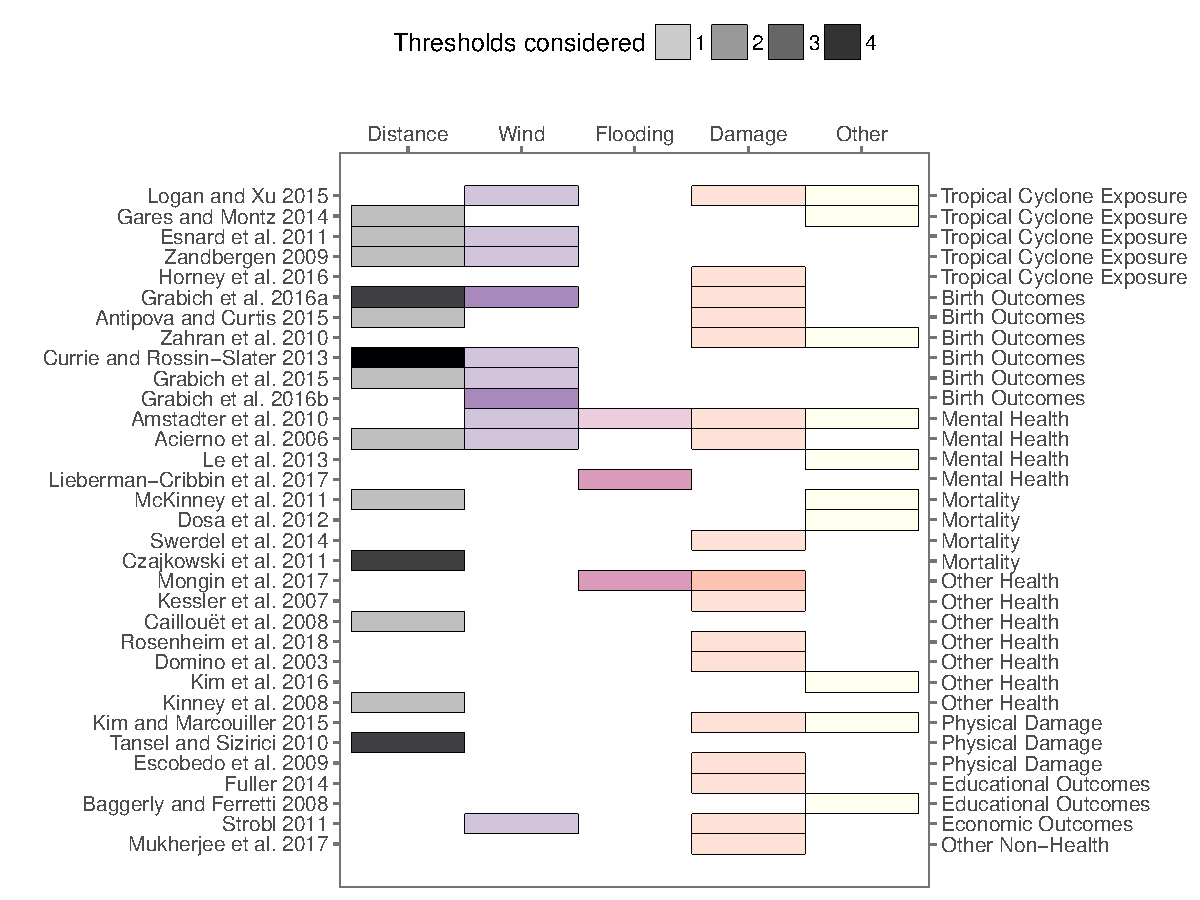
\includegraphics[width=\linewidth]{previous_exposure_metrics}
\caption{Metrics used in a sample of previous studies to assign exposure to tropical cyclones in U.S.-based tropical cyclone exposure or impact studies. Citations for each study are shown on the left and the broad topic of the study on the left. Presence of a bar for a study-metric combination indicates that the given metric was used in the study in assessing exposure to tropical cyclones for that study, either alone or in combination with other metrics for which that study has bars. The color transparency of each bar indicates the number of different thresholds considered for defining storm exposure in the study under that hazard (e.g., less transparent bars indicate that a study considered multiple thresholds of the metric in defining tropical cyclone exposure as a method of sensitivity analysis). Studies for which there are two or more bars (e.g., bars for both distance and wind) indicate studies that either used separate exposure assessments, one for each metric, (e.g., as a sensitivity analysis) or used a single exposure index that incorporated multiple metrics in its definition. ``Damage" often indicate use of Federal Emergency Management Agency (FEMA) reports, although occasionally used damage reports from other sources, including newspaper reports. Examples of ``Other" include evacuation orders, excessive school closures, length of time a storm was near a location, and detailed, holistic analyses of a specific storm or storms. References for each study are included in the
bibliography of this Supplemental Material.}
\label{fig:previousmetrics}
\end{figure}

\nocite{logan2015, gares2014, esnard2011, zandbergen2009, horney2016, grabich2016, 
antipova2015post, zahran2010, currie2013, grabich2015, grabich2016hurricane, amstadter2010,
acierno2006, le2013, lieberman2017, mckinney2011, dosa2012evacuate, swerdel2014, 
czajkowski2011, mongin2017, kessler2007hurricane, caillouet2008increase, 
rosenheim2018disaster, domino2003disasters, kim2016, kinney2008, kim2015, tansel2010,
escobedo2009, fuller2014, baggerly2008impact, strobl2011economic, mukherjee2017}

\newpage

\begin{figure}[tbhp!]
\centering
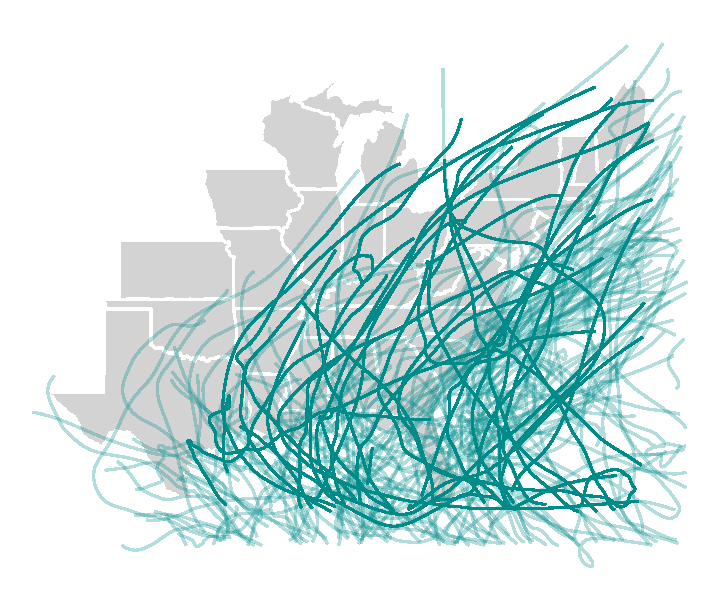
\includegraphics[width=0.7\linewidth]{hurrtracks}
\caption{Tracks of all tropical cyclones included in the study. The study included all tracked storms in the revised Atlantic hurricane database (HURDAT2 \citep{landsea2013}) that came within 250 kilometers of at least on U.S. county, 1988--2015. Thicker lines show the tracks of storms whose names were retired, indicating that the storm was particularly severe or had notable impacts \citep{retirednames}.}
\label{fig:hurrtracks}
\end{figure}

\clearpage

\begin{figure}[tbhp!]
\centering
\includegraphics[width=\linewidth]{othertopstorms}
\caption{Counties exposed, based on different exposure metrics, to the storms with largest extent (as measured by the number of counties exposed based on any metric) from each of the clusters shown in the Jaccard heatmap in the main text (Figure 2).}
\label{fig:othertopstorms}
\end{figure}

\clearpage

\begin{figure}[tbhp!]
\centering
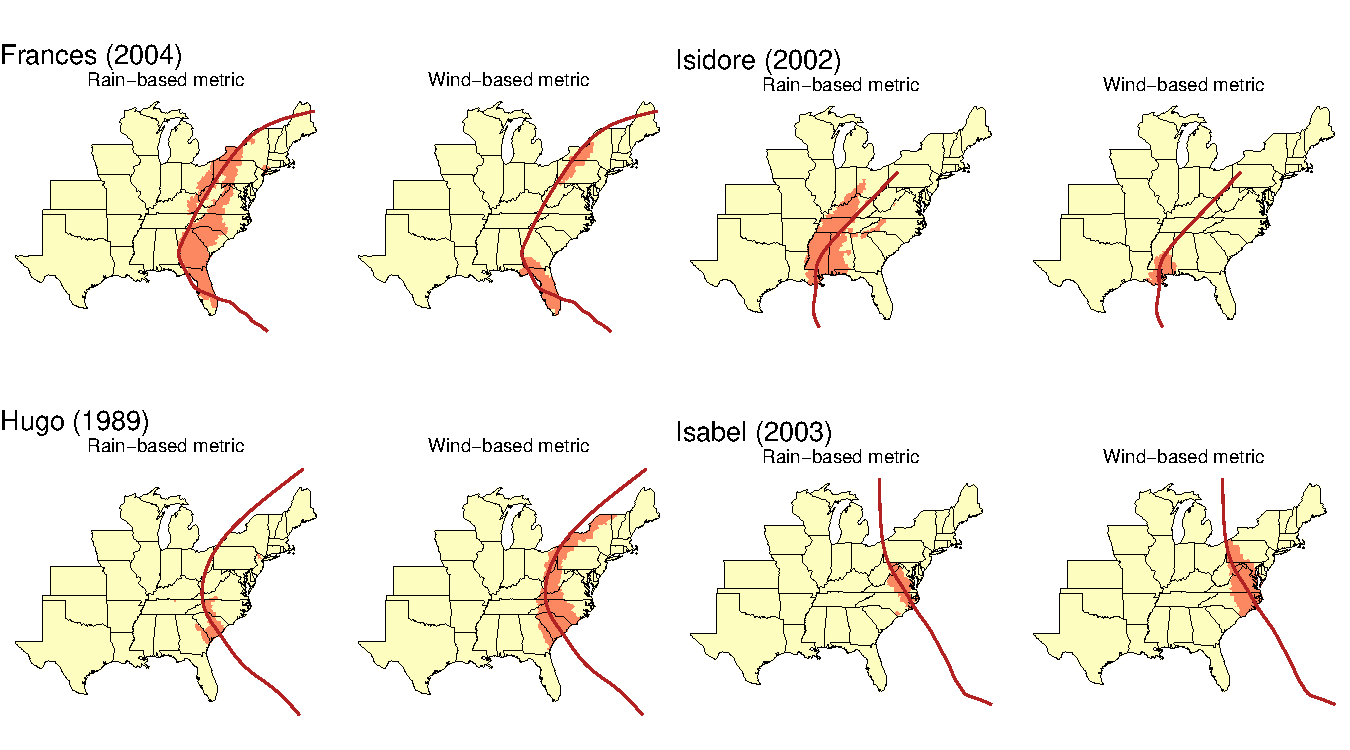
\includegraphics[width=\linewidth]{extentdisagreement}
\caption{Examples of storms for which exposure assessments differed substantially between rain-based and wind-based metrics. Counties shown in orange were classified as exposed to a given storm by a given metric; those in yellow were classified as not exposed. The storm's track is shown in red. For both Frances (2004) and Isidore (2002) (top panel), substantially more counties were assessed as exposed when measuring exposure based on rain rather than wind. Conversely, for both Hugo (1989) and Isabel (2003) (bottom panel), substantially more counties were assessed as exposed based on wind compared to rain.}
\label{fig:extentdisagreement}
\end{figure}

\clearpage

\begin{figure}[tbhp!]
\centering
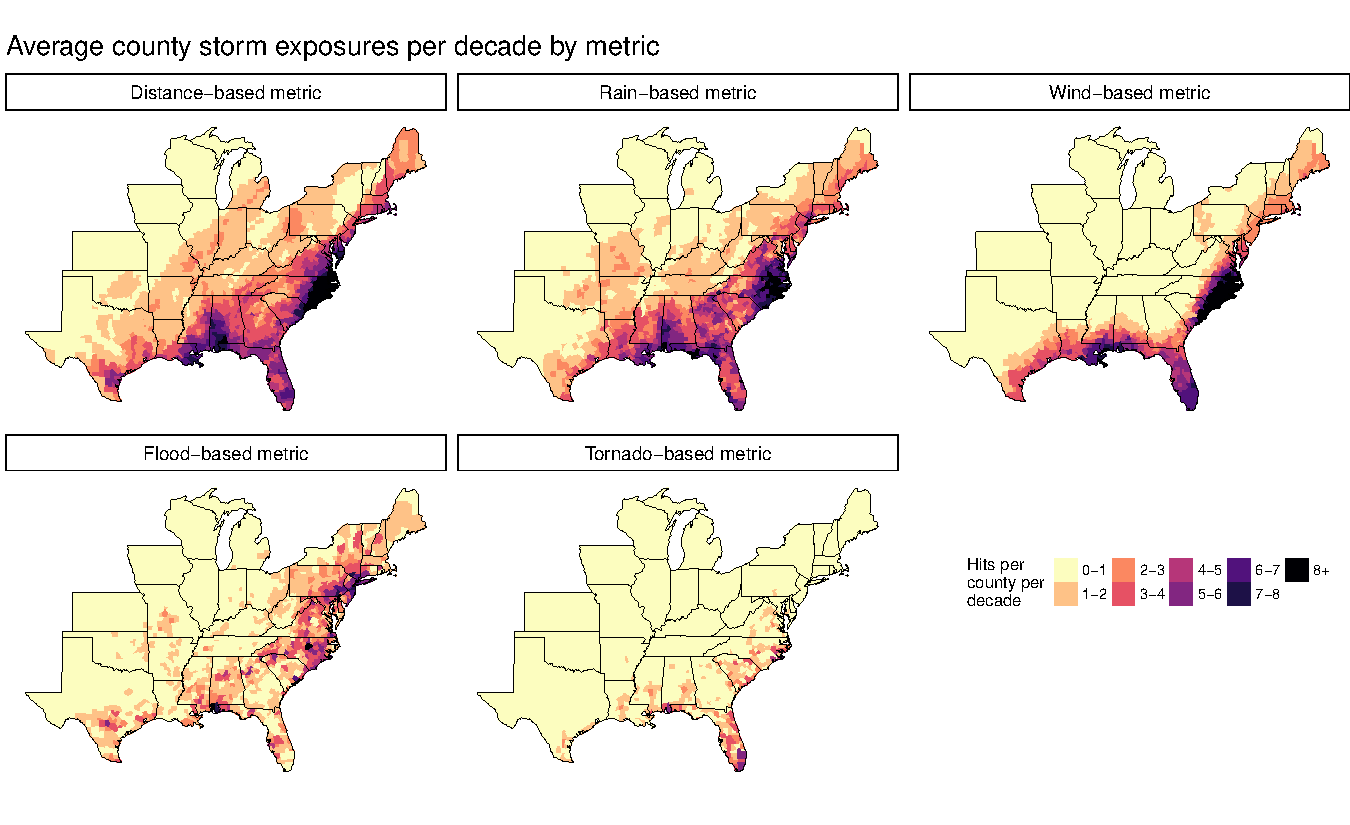
\includegraphics[width=\linewidth]{averageexposureonlysupp}
\caption{Average number of storm exposure per decade in U.S. counties for each exposure metric, based on years of for which data for all five exposure metrics are available (1996--2011). The criteria behind each of the five metrics is given in Table 1 of the main text.}
\label{fig:averageexposuresupp}
\end{figure}

\clearpage

\begin{figure*}%[tbhp]
\centering
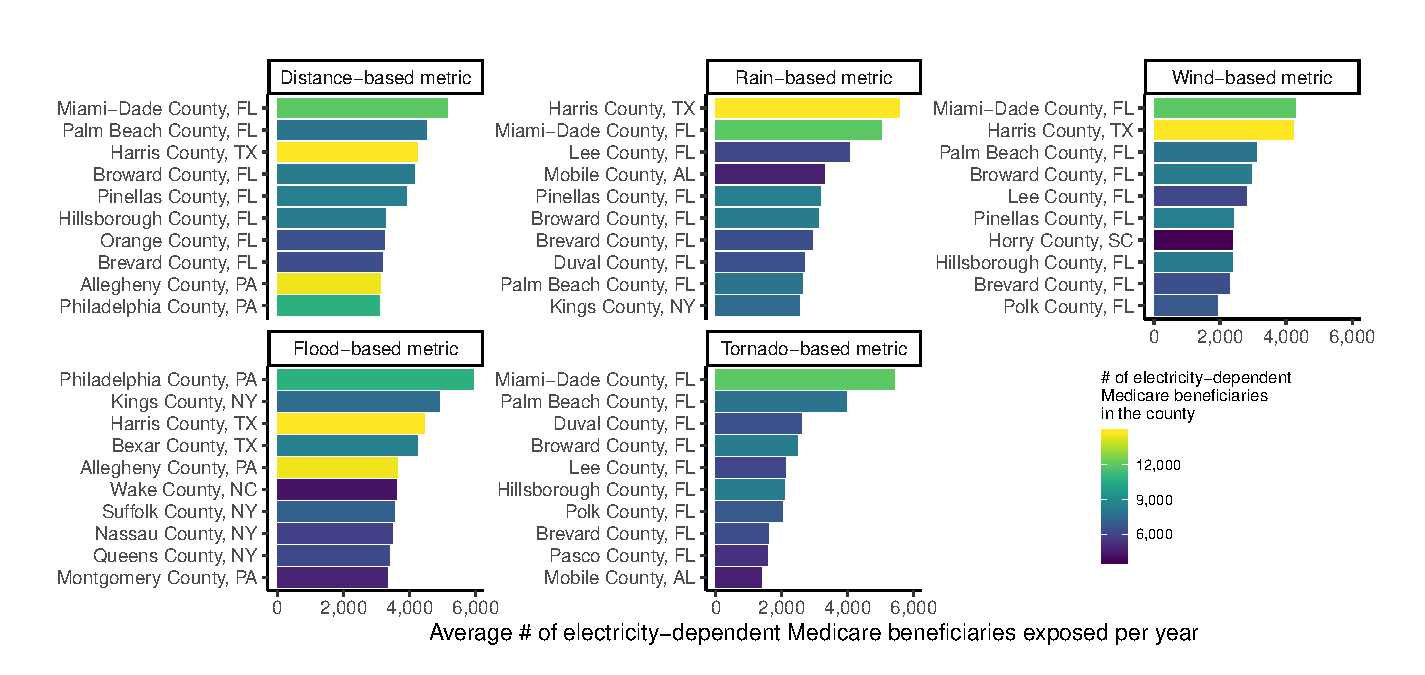
\includegraphics[width=15.5cm]{topelecdependexposure}
\caption{Counties with the highest estimated physical exposure among electricity-dependent Medicare beneficiaries exposed to storms per year in U.S. counties for each exposure metric. The criteria behind each of the five metrics is given in Table 1 of the main text and details of the physical exposure calculation are given in the Methods. The color of each bar indicates the number of Medicare beneficiaries in the county reliant on electricity-dependent medical and assistive equipment as of July 2017 \citep{empower}. The length of each bar shows the average expected number of these electricity-dependent Medicare beneficiaries exposed to tropical storms per year based on a given exposure metric.}
\label{fig:topelecdependexposure}
\end{figure*}

\clearpage

\begin{figure}[tbhp!]
\centering
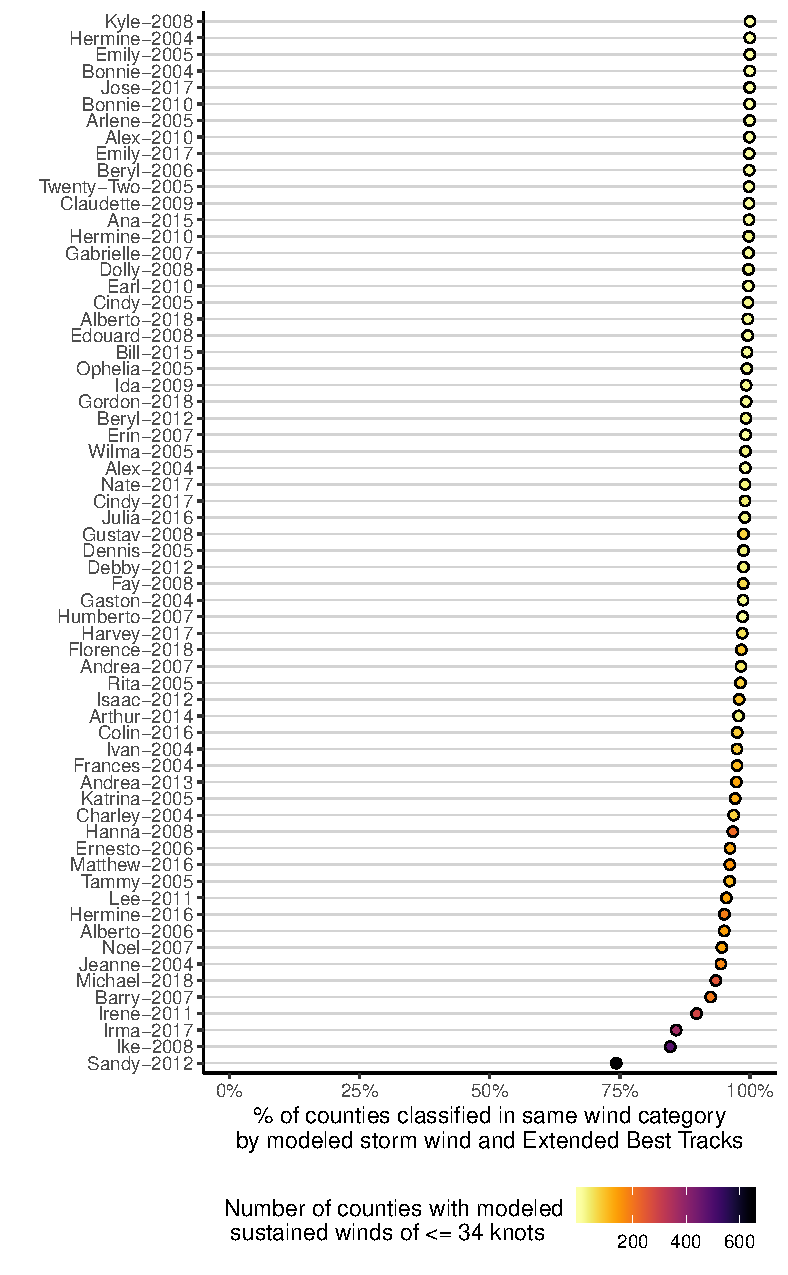
\includegraphics[width=0.6\linewidth]{windcomparison}
\caption{Comparison of estimated wind categories from modeled sustained wind speed (as used for the wind exposure metric in the main text; \citep{stormwindmodel}) versus sustained wind speed determined from the revised Atlantic hurricane database (HURDAT2 \citep{landsea2013}). In HURDAT2, wind radii were available for study storms from 2004--2015 and gives estimates of the maximum radii to which storm winds of 34 knots, 50 knots, and 64 knots extended in each four quadrant of the storm at each of the six-hour storm track observations. We interpolated this data to 15-minute increments and assessed a county as exposed to winds at or above one of these cutoffs if its population mean center was within 85\% of the maximum radius for that wind speed in its quadrant of the storm. For each county in each of the available storms, we also calculated the modeled wind speed \citep{stormwindmodel} and then categorized this value into the same categories available for the HURDAT2 wind radii ($<$34 knots; 34--49.9 knots; 50--63.9 knots; $\ge$64 knots). Each point in this graph shows, for a storm, the percent of counties in which the wind category ($<$34 knots; 34--49.9 knots; 50--63.9 knots; $\ge$64 knots) was the same based on both modeled winds and the HURDAT2 wind radii. Only storms with at least one county with sustained wind of $\ge$34 knots, based on the HURDAT2 wind radii, are shown. Hurricanes Sandy (2012) and Ike (2008) were he two storms with the worst agreement between these two sets of wind data; maps with further comparisons between the two data sources for these two storms are given in Fig. \ref{fig:windexamples}.}
\label{fig:windcomparison}
\end{figure}

\begin{figure}[tbhp!]
\centering
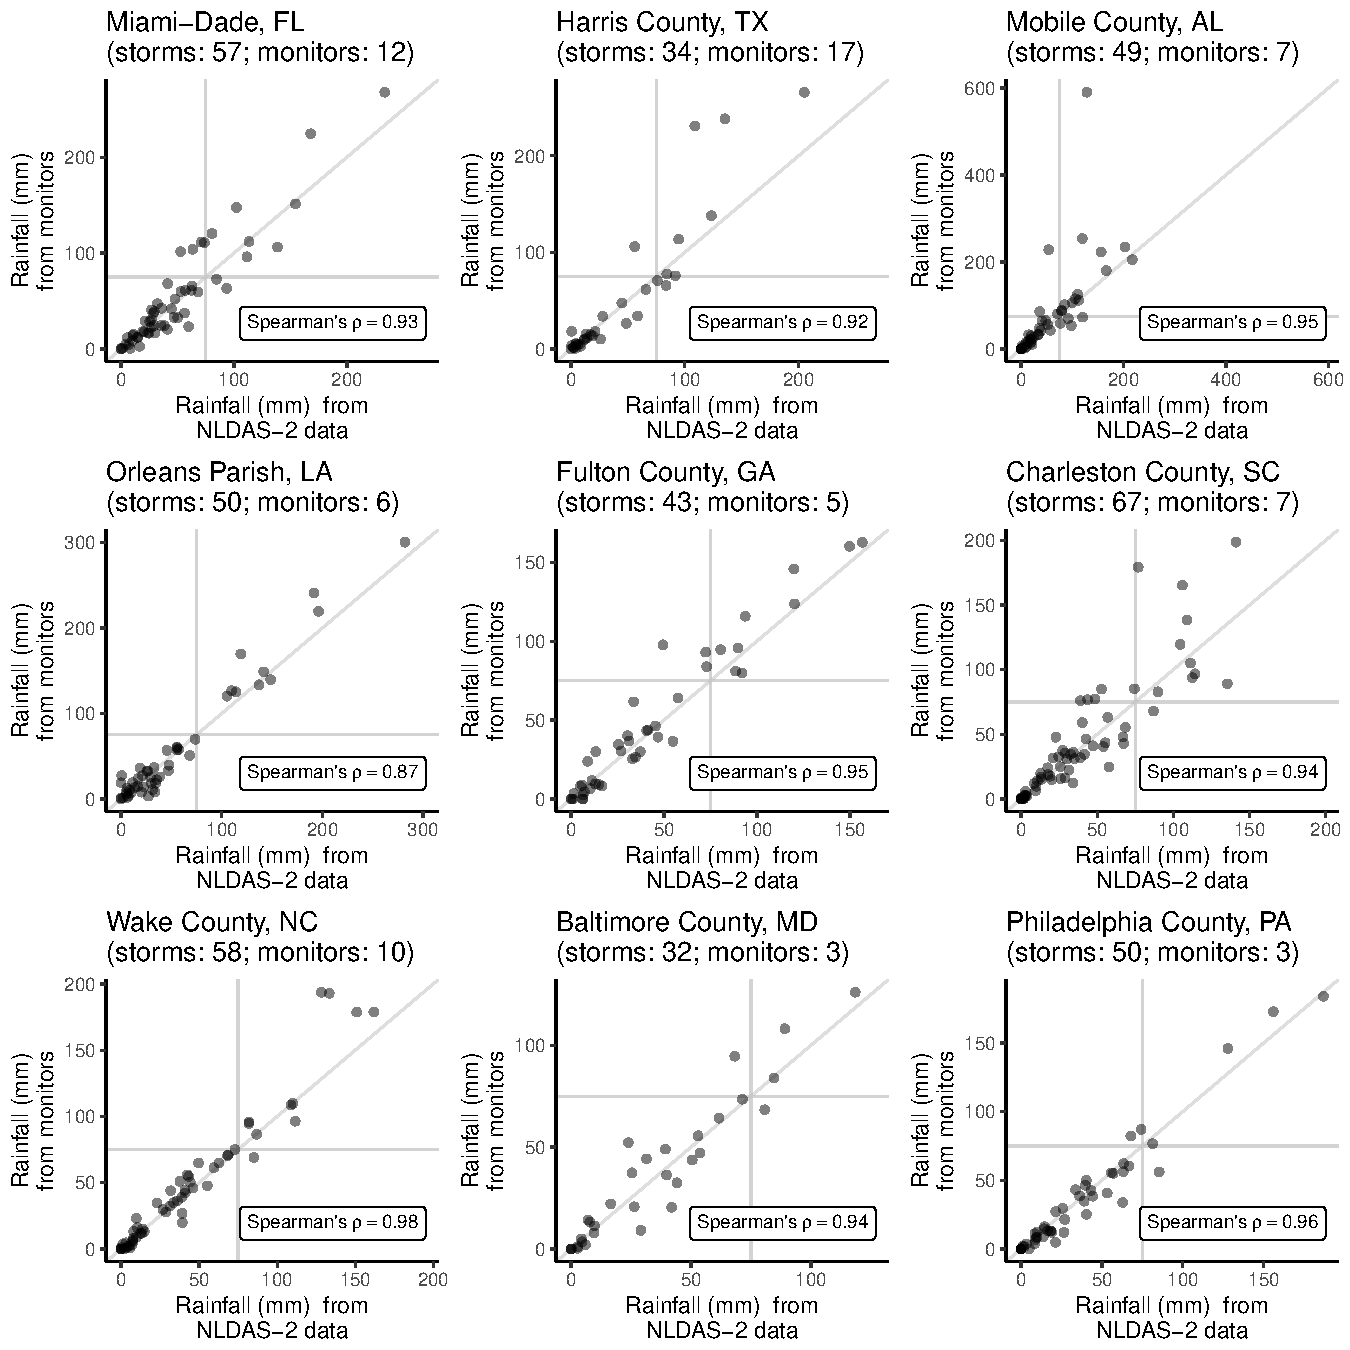
\includegraphics[width=0.9\linewidth]{raincomparison}
\caption{Comparison of county-level rain exposure based on the reanalysis data used for exposure assessment in this study (NLDAS-2) \citep{rui2013nldas, alhamdan2014environmental} and ground-based weather stations \citep{menne2012overview, rnoaa, countyweather}. Each small graph shows a sample county, and each point on the graph represents a tropical storm that came within 500 kilometers of the population mean center of the county. The x-axis shows the estimated cumulative rainfall (in millimeters) from two days before to one day after the storm's closest approach to the county based on the county-aggregated NLDAS-2 precipitation data used to measure rain exposure in our main analysis. The ground-based observations (y-axis) are based on collecting precipitation data from available weather stations in the county, 1988--2011, summed over the same period from two days before to one day after the storm's closest approach for each available station. These cumulative station-based precipitation totals were then averaged across all available stations in the county to create a county-wide estimate of cumulative storm-related precipitation for each storm in the county. Horizontal and vertical lines show the threshold used to classify a storm as exposed based on cumulative rainfall; storms in the lower left and upper right quadrants are classified the same regardless of whether reanalysis or station-based precipitation data is considered, while storms in the upper left and lower right quadrants would be classified differently. The number of storms within each county and the average number of stations reporting rainfall during the county's storms are given above each plot. Note that x- and y-axis ranges differ by county. An estimate of the rank correlation (Spearman's $\rho$ \citep{spearman1904proof}) between measurements from the two rain data sources is also shown on each graph.}
\label{fig:raincomparison}
\end{figure}

\begin{figure}[tbhp!]
\centering
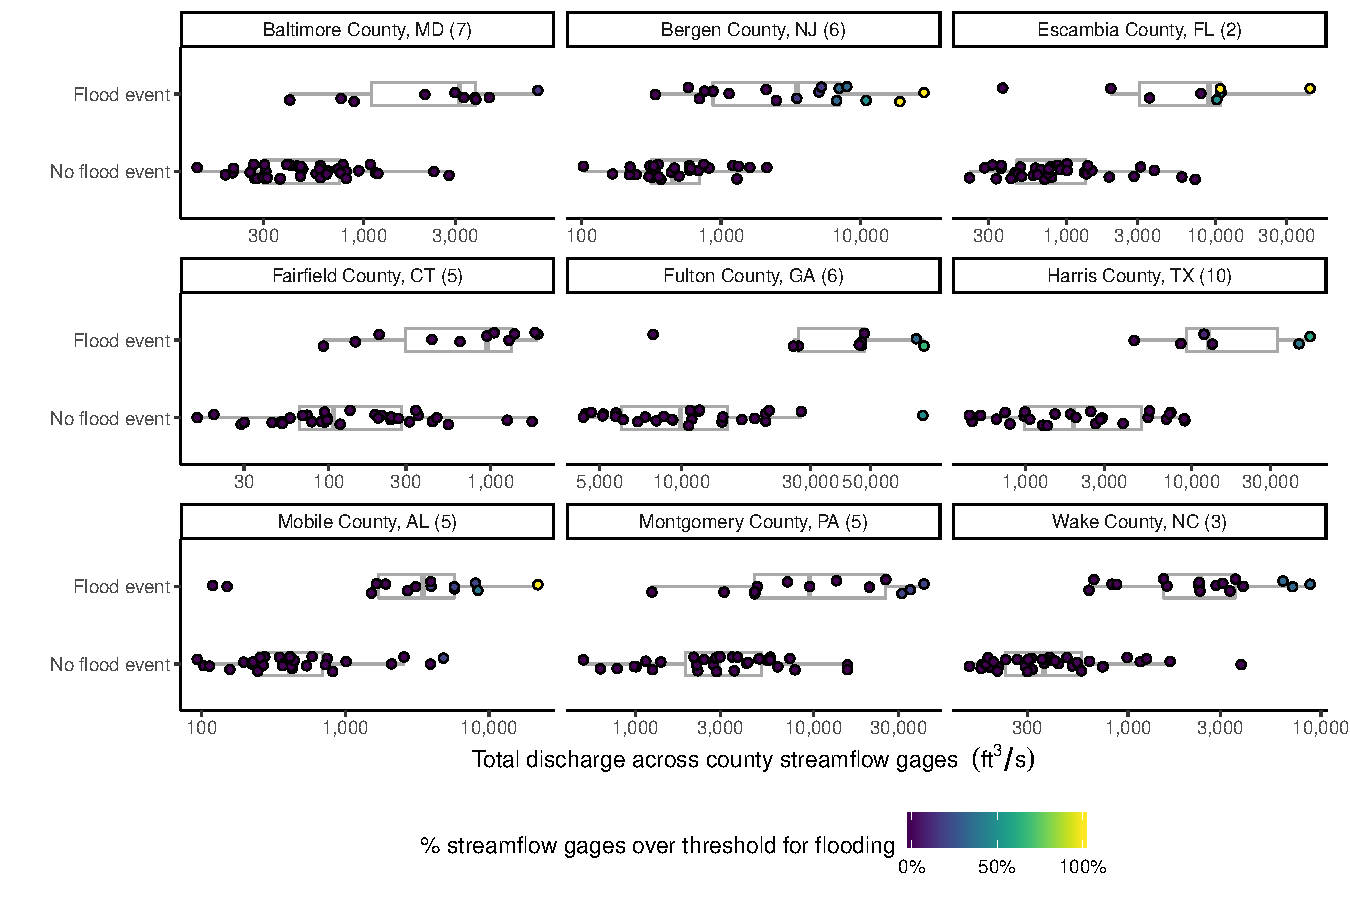
\includegraphics[width=0.8\linewidth]{floodcomparison}
\caption{Comparison of for a sample of study counties of flood status, based on NOAA Storm Events listings \citep{stormevents, noaastormevents}, with total streamflows at county streamflow gages during tropical storms \citep{usgsgages, countyfloods, dataRetrieval}. Each panel represents a separate county. For each county, we first identified all streamflow gages in the county that had complete data for Jan. 1 1996--Dec. 31, 2015. The number of streamflow gages meeting this criterion are given in parentheses beside the county's name in the panel title. This analysis covered tropical storm that came within 500 kilometers of each sample county between 1996 and 2015. In the graphs, each point represents a single tropical storm, and the point's position along the x-axis shows the highest daily total streamflow (cubic feet / second), summed across all identified streamgages in the county, for a five-day window centered on the day of the storm's closest approach to the county. The y-axis separates storms for which a flood event was reported in NOAA's Storm Events database for the county with a start date within the five-day window of the storm's closest approach to the county \citep{stormevents, noaastormevents}. Boxplots are added to show the distribution of the total streamflow measurements across storms in the county for storms grouped by whether or not they were linked with a flood event based on the NOAA Storm Events data. The color of each point gives the percent of streamflow gages in the county with a daily streamflow that exceeded a threshold of flooding (the streamgage's median value for annual peak flow \citep{countyfloods}) on any day during the five-day window.  Note that the x-axis scales differ by county, depending on the number of streamflow gages and typical flow rates for each gage, and are on a log-10 scale.}
\label{fig:floodcomparison}
\end{figure}

\begin{figure}[tbhp!]
\centering
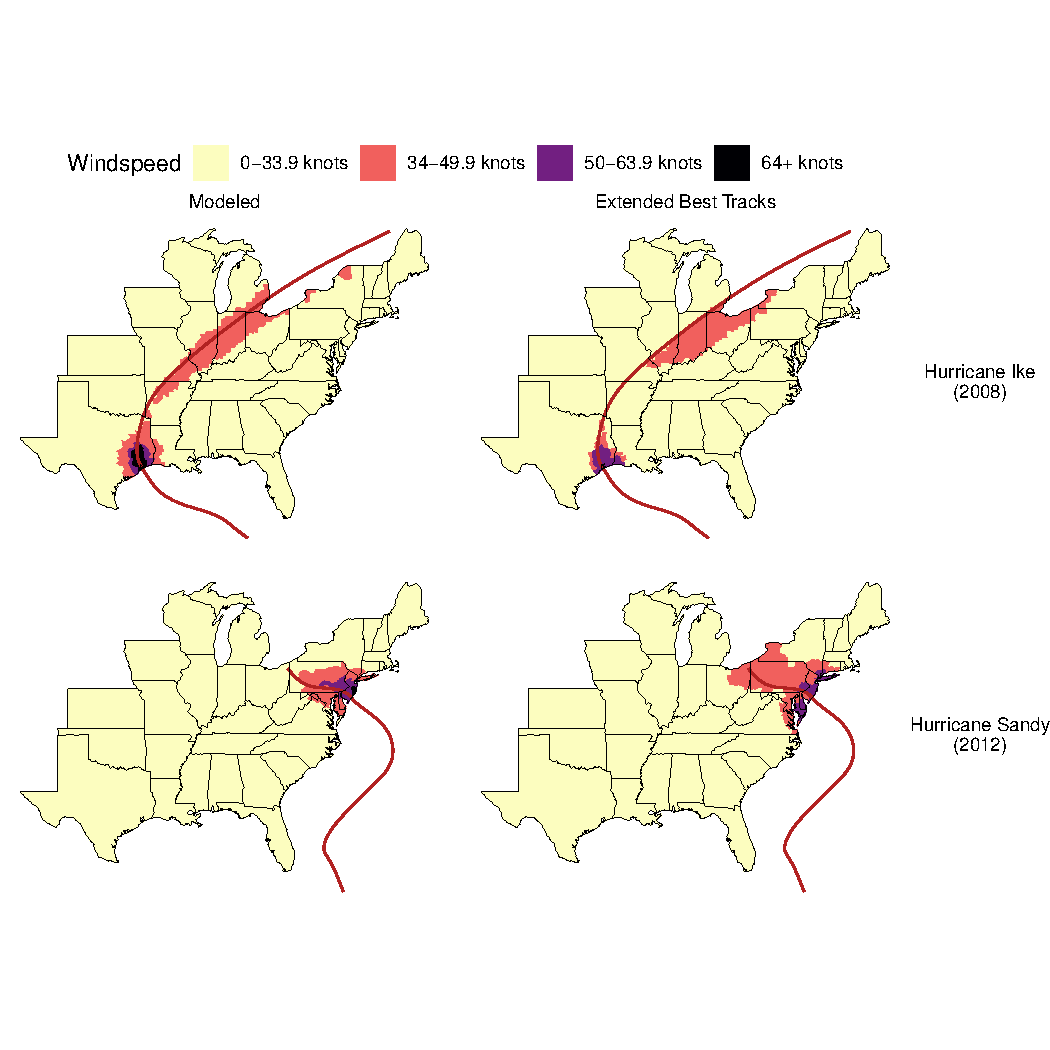
\includegraphics[width=\linewidth]{windexamples}
\caption{Wind classifications for the two storms, Hurricanes Sandy (2012) and Ike (2008) for which exposure classifications from modeled wind data \citep{stormwindmodel} and HURDAT2 wind radii \citep{demuth2006improvement} showed the highest disagreement for storms between 2004 and 2015 (Fig. \ref{fig:windcomparison}). The top two maps show modeled (left) and HURDAT2 (right) windspeed categorizations for Hurricane Ike (2008), while the bottom two maps show the same windspeed characterizations for Hurricane Sandy (2012). In both cases, the storms were exceptionally large systems for which high winds persisted well inland from landfall and for which, based on the HURDAT2 data, a large number of counties were exposed to winds of $\ge$34 knots (Figure \ref{fig:windcomparison}).}
\label{fig:windexamples}
\end{figure}

\begin{figure}[tbhp!]
\centering
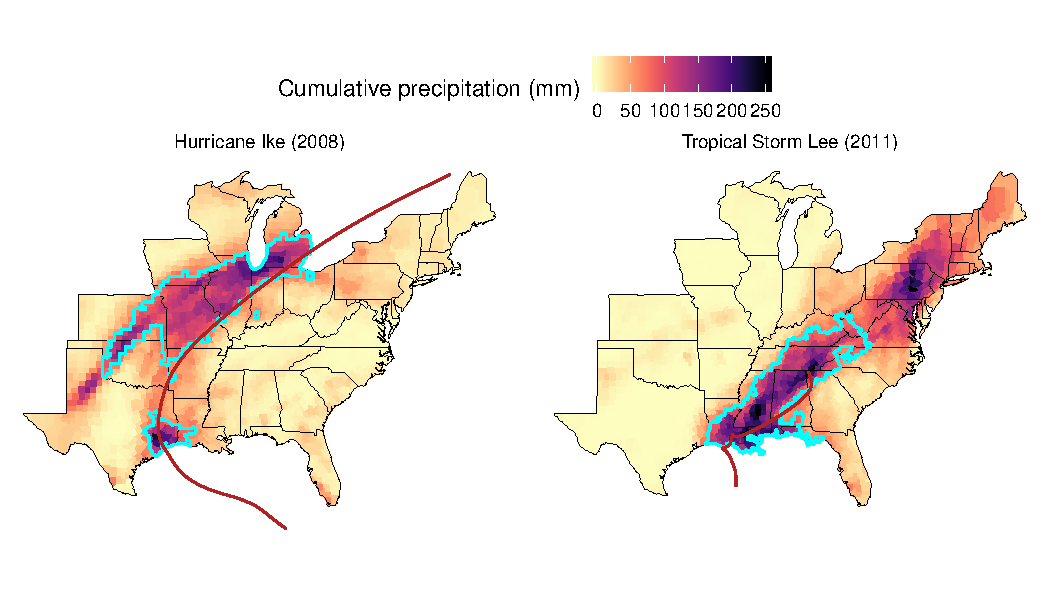
\includegraphics[width=0.9\linewidth]{rainexamples}
\caption{Examples of storms where the rain exposure classification method fails to capture full storm-related rainfall because of the distance constraint used in that assessment metric. The red line on each map shows the track of the storm, based on the revised Atlantic hurricane database (HURDAT2 \citep{landsea2013}). The color of each county in the map gives the cumulative precipitation (in millimeters) for that county during the window from two days before to one day after the storm's closest approach to the county. The blue outline identifies the collection of counties that were classified as ``exposed" based on the criteria that the storm passed within 500 kilometers of the county's population mean center and the cumulative rainfall was 75 millimeters or more (Table 1 of main text). The map on the left shows rain-based exposure for Hurricane Ike. For this exceptionally large storm, there are some counties in northern Texas that received high rainfall from the storm but are too far from the storm center's track to be classified as exposed by this metric. The map on the right shows rain-based exposure for Tropical Storm Lee. For this storm, rain from the storm affected counties in the Mid-Atlantic and New England as the remnants of the storm moved over those regions, but storm tracking stopped while the storm was still over the southeastern part of the U.S., and so these counties are not classified as exposed to the storm based on this metric.}
\label{fig:rainexamples}
\end{figure}

\clearpage



\bibliography{hurr_exposure}

\end{document}
